\documentclass{article}
\usepackage[utf8]{inputenc}
\usepackage[shortlabels]{enumitem}
\usepackage{geometry}
\geometry{a4paper,left=20mm,right=20mm, top=10mm}
\usepackage{graphicx}
\usepackage{float}
\usepackage{amsmath}
\usepackage{bm}
\usepackage{dsfont}
\usepackage{upgreek}
\usepackage{float}
\usepackage{xcolor}
%\usepackage{color}
\usepackage{subcaption}
\usepackage{graphicx} 
\usepackage{hyperref}
\usepackage{tikz}
\usetikzlibrary{arrows}
\usepackage{array}
\setlength\parindent{0pt}
\usepackage{multirow}
\usepackage{makecell}

\renewcommand\cellalign{cl}
\begin{document}

Model 1: Forward direction is in red, backward direction is in black, observations are in bold:

\begin{table}[H]
\centering
\begin{tabular}{|c|c|c|c|c|}
	\hline
	$\mathbf{h_{1n}}:$ & $g_1(x_n)$ & $\color{red} h_{13}(g_3(x_n))$ & $\color{red} h_{12}(g_2(x_n))$ & $\color{red} h_{123}(h_{23}(g_3(x_n)))$\\
	\hline
	$\mathbf{h_{2n}}:$ & $g_2(x_n)$ & $h_{21}(g_1(x_n))$ & $\color{red} h_{23}(g_3(x_n))$\\
	\hline
	$\mathbf{h_{3n}}:$ & $g_3(x_n)$ & $h_{31}(g_1(x_n))$ & $h_{32}(g_2(x_n))$ & $ h_{321}(h_{21}(g_1(x_n)))$\\
	\hline
	
\end{tabular}
\end{table}

The number of GPs will explode as the Pascal's Triangle.\\

For Model 1 forward version:

\begin{figure}[H]
\centering
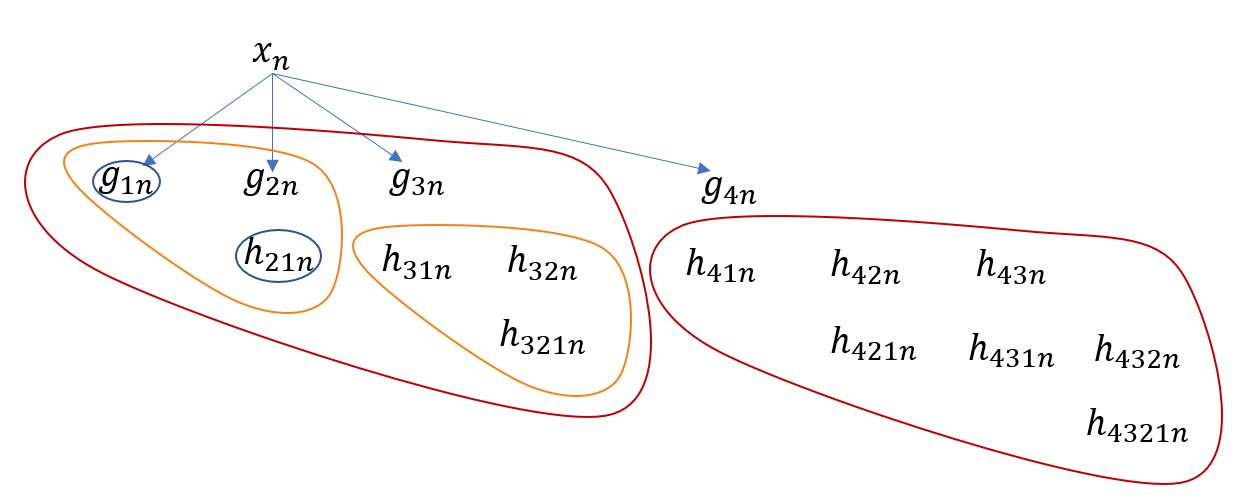
\includegraphics[width=0.7\textwidth]{new2.png}
\end{figure}

\begin{align*}
	p(\mathbf{y},g_{1:3}, h_{21,31,32,321}) = &  p(g_{1\neq\mathbf{u}_1}|\mathbf{u}_1)p(g_{2\neq\mathbf{u}_2}|\mathbf{u}_2)p(g_{3\neq\mathbf{u}_3}|\mathbf{u}_3)p(\mathbf{u}_1)p(\mathbf{u}_2)p(\mathbf{u}_3)\\	
	& p(h_{21\neq\mathbf{v}_1}|\mathbf{v}_1)p(h_{31\neq\mathbf{v}_2}|\mathbf{v}_2)p(h_{32\neq\mathbf{v}_3}|\mathbf{v}_3)p(\mathbf{v}_1)p(\mathbf{v}_2)p(\mathbf{v}_3)\\	
    & p(h_{321\neq\mathbf{w}_1}|\mathbf{w}_1)p(\mathbf{w}_1)\\
    & \prod_n p(y_{1n};g_1(x_n), \sigma^2_1)\\
    & \hspace{1.5em} p(y_{2n};g_2(x_n) + h_{21}(g_1(x_n)), \sigma^2_2)\\
    & \hspace{1.5em} p(y_{3n};g_3(x_n) + h_{31}(g_1(x_n)) + h_{32}(g_2(x_n)) + h_{321}(h_{21}(g_1(x_n))), \sigma^2_3)
\end{align*}

\begin{align*}
	q(g_{1:3}, h_{21, 31, 321}) = & p(g_{1\neq\mathbf{u}_1}|\mathbf{u}_1)p(g_{2\neq\mathbf{u}_2}|\mathbf{u}_2)p(g_{3\neq\mathbf{u}_3}|\mathbf{u}_3)q(\mathbf{u}_1)q(\mathbf{u}_2)q(\mathbf{u}_3)\\
	& p(h_{21\neq\mathbf{v}_1}|\mathbf{v}_1)p(h_{31\neq\mathbf{v}_2}|\mathbf{v}_2)p(h_{32\neq\mathbf{v}_3}|\mathbf{v}_3)q(\mathbf{v}_1)q(\mathbf{v}_2)q(\mathbf{v}_3)\\	
	& p(h_{321\neq\mathbf{w}_1}|\mathbf{w}_1)q(\mathbf{w}_1)\\
\end{align*}

\begin{align*}
	\mathcal{L}_{ELBO} = & \mathds{E}_q\left[ \frac{p(\mathbf{y},g_{1:3}, h_{21,31,32,321})}{q(g_{1:3}, h_{21, 31, 321})}\right]\\
	=  & \sum_n \int q(g_{1n}|x_n) \log p(y_{1n}|g_{1n}, \sigma^2_1) \\
	& + \sum_n \int q(g_{1n}|x_n) q(g_{2n}|x_n) q(h_{21n}|g_{1n}) \log p(y_{2n}|g_{2n},h_{21n},\sigma^2_2) \\
	& + \sum_n \int q(g_{1n}|x_n)  q(g_{2n}|x_n) q(g_{3n}|x_n)\\
	& \hspace{4em} q(h_{21n}|g_{1n}) q(h_{31n}|g_{1n}) q(h_{32n}|g_{2n}) q(h_{321n}|h_{21n}) \log p(y_{3n}| g_{3n}, h_{31n}, h_{32n}, h_{321n}, \sigma^2_3)\\
	& -\sum_{\mathbf{u}: \text{\footnotesize all inducing points}} KL(q(\mathbf{u})\|p(\mathbf{u}))
\end{align*}

where $q(\cdot|\cdot)$ is the variational posterior with inducing points analytically marginalized out. The following table shows the space where each GP's inducing inputs should lie.

\begin{table}[H]
\centering
\begin{tabular}{|c|c|c|c|}
\hline
$g_{1:3}$ & $\mathcal{X}$\\
$h_{21,31}$ & $g_1(\mathcal{X})$\\
$h_{32}$ & $g_2(\mathcal{X})$\\
$h_{321}$ & $h_{21}(g_2(\mathcal{X}))$\\
\hline
\end{tabular}
\end{table}

If bi-directional is implemented, the expectation log-term will be:

\begin{align*}
	& \sum_n \int q(g_{1n}|x_n)q(g_{2n}|x_n)q(g_{3n}|x_n)\\
	& \hspace{4em} \bigg[ \int  q(h_{13n}|g_{3n}) q(h_{12n}|g_{2n}) q(h_{23n}|g_{3n}) q(h_{123n}|h_{23n}) \log p(y_{1n}|g_{1n}, h_{13n}, h_{12n}, h_{123n}, \sigma_1^2)\\
	& \hspace{4em} \int q(h_{21n}|g_{1n}) q(h_{23n}|g_{3n}) \log p(y_{2n}|g_{2n}, h_{21n}, h_{23n}, \sigma^2_2)\\
	& \hspace{4em} \int q(h_{21n}|g_{1n}) q(h_{31n}|g_{1n}) q(h_{32n}|g_{2n}) q(h_{321n}|h_{21n}) \log p(y_{3n}| g_{3n}, h_{31n}, h_{32n}, h_{321n}, \sigma^2_3) \bigg]
\end{align*}

The above model can also be relaxed as Model 2:
\begin{table}[H]
\centering
\begin{tabular}{|c|c|c|c|c|c|c|}
	\hline
	$t_{1n}:$ & & & $\color{blue} g_1(x_n)$ & $\color{red} g_{13}(b_{3n})$ & $\color{red} g_{12}(b_{2n})$  & $:b_{1n}$\\
	\hline
	$t_{2n}:$ & & $g_{21}(t_{1n})$ & $\color{blue} g_2(x_n)$ & $\color{red} g_{23}(b_{3n})$ &  & $:b_{2n}$\\
	\hline
	$t_{3n}:$ &$g_{32}(t_{2n})$ & $g_{31}(t_{1n})$ & $\color{blue} g_3(x_n)$ &  &  & $:b_{1n}$\\
	\hline
\end{tabular}
\end{table}

where the hidden variables in two directions share the GP over input as follows,

\begin{align*}
	t_{1n} &= g_1(x_n)\\
	t_{2n} &= g_2(x_n) + g_{21}(t_{1n})\\
	t_{3n} &= g_3(x_n) + g_{32}(t_{2n}) + g_{31}(t_{1n})\\
	\\
	b_{3n} &= g_3(x_n)\\
	b_{2n} &= g_2(x_n) + g_{23}(b_{3n})\\
	b_{3n} &= g_1(x_n) + g_{12}(b_{2n}) + g_{13}(b_{3n})\\
	\\
	h_{1n} &= g_1(x_n) + g_{12}(b_{2n}) + g_{13}(b_{3n})\\
	h_{2n} &= g_2(x_n) + g_{21}(t_{1n}) + g_{23}(b_{3n})\\
	h_{3n} &= g_3(x_n) + g_{32}(t_{2n}) + g_{31}(t_{1n})
\end{align*}

Just like Model 1, Model 2's backwards direction does not have any duplicated function over time. The number of GPs is $L^2$, where $L$ is number of outputs. However, the dependencies will still run through aggregated hidden variables, except that time and each previous output are explicitly separated.\\

Here is the connection of all three model:

\begin{figure}[H]
\centering
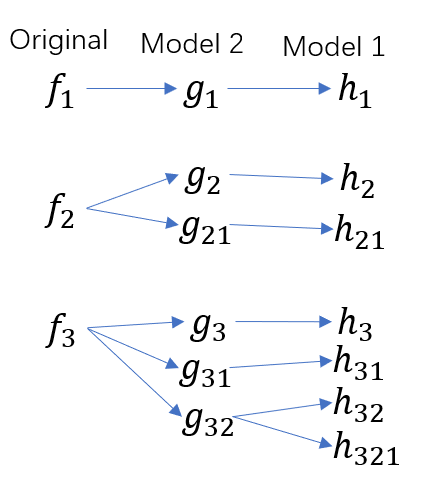
\includegraphics[width=0.3\textwidth]{new3.png}

\end{figure}



\end{document}


